\documentclass[titlepage]{article}
\usepackage[utf8]{inputenc}
\usepackage{bera}
\usepackage{listings}
\usepackage{color}
\usepackage{epigraph}
\usepackage[all]{genealogytree}
\usepackage{enumitem}
\usepackage{amsmath}
\usepackage{csquotes}
\usepackage{url}
\usepackage{hyperref}
\hypersetup{
    colorlinks=false
}
\urlstyle{same}

\usepackage[boxed,linesnumbered,algo2e]{algorithm2e}
\usepackage{qtree}
% \usepackage{array}
% \usepackage{tikz-qtree}

% \usepackage[backend=biber]{biblatex}
% \addbibresource{bibliography_outlab_6.bib}

\renewcommand{\labelitemi}{\large \textbullet}
% \newcommand*{\marriage}[2]{
% \begin{tabular}{>{\raggedleft}p{.5in}@{}>{\centering}p{.2in}@{}>{}p{.5in}}%
% #1 & \rule[3pt]{.2in}{\pgflinewidth} & #2
% \end{tabular}}


\begin{document}

\title{ \huge {\textbf{Software Systems Lab: OutLab \\ Advanced \LaTeX}}}
\author{Contour \\ 160050002 \\ 160050056 \\ 160050057}
\date{22 August, 2017}
\maketitle

\tableofcontents

\newpage

You need to replicate this document

\section{\textbf{Do this}}

\begin{itemize}
    \setlength\itemsep{2em}
    \item {\LaTeX} typesets a file of text using the TEX program.
    \item {\LaTeX} is widely used in academia for the communication and publication of scientific documents in many fields, including mathematics, physics, computer science, statistics, economics and political science.
    \item {\LaTeX} can be used as a standalone document preparation system or as an intermediate format.
    \item \textbf{Have used renewcommand for the bullets to be bigger.}
    \item look at the item separation space, and change it accordingly
\end{itemize}
\begin{enumerate}[label*=\Roman*]
    \setlength{\itemindent}{-1em}
    \item {\LaTeX} typesets a file of text using the TEX program.
    \item {\LaTeX} is widely used in academia for the communication and publication of scientific documents in many fields, including mathematics, physics, com- puter science, statistics, economics and political science.
    \item   {\LaTeX} can be used as a standalone document preparation system or as an intermediate format.
    \item {\LaTeX} is intended to provide a high-level language that accesses the power of TeX in an easier way for writers.
\end{enumerate}

\begin{enumerate}[label*=(\alph*)]
    \setlength{\itemindent}{-1em}
    \item {\LaTeX} typesets a file of text using the TEX program.
    \item {\LaTeX} is widely used in academia for the communication and publication of scientific documents in many fields, including mathematics, physics, com- puter science, statistics, economics and political science.
\end{enumerate}

\section{\textbf{Mathematical Formulas and notations}}

\subsection{Equation Array}
\begin{eqnarray}
cos^3 \theta + sin^3 \theta & = & (cos\theta + sin\theta)(cos2\theta - cos\theta sin\theta \\
                    & = & (cos\theta + sin\theta)(1-cos\theta sin\theta) \\
                    & = & (cos\theta + sin\theta)(1/2)(2-2cos\theta sin\theta)(3) \\
                    & = & (1/2)(cos\theta + sin\theta)(2-sin(2\theta ))
\end{eqnarray}

\subsection{Prepositional Formulae using Various Operators}
\begin{flalign*}
&(\exists x)(\varphi (x) \Lambda \psi (x)) \longleftrightarrow ((\exists x)\varphi x \Lambda (\exists x)\psi (x))& \\
&((\forall x)\varphi (x) \Lambda (\forall x) \psi (x)) \longrightarrow (\forall x)(\varphi (x) \Lambda \psi (x))& \\
&(\exists x)(\varphi (x) \Lambda \psi(x)) \longrightarrow ((\exists x)\varphi(x) \Lambda (x)(\exists x) \varphi(x) \Lambda (\exists x)\psi(x))&
\end{flalign*}
\subsection{Alphabets}
\begin{center}
%\bgroup
%\def\arraystretch{2}
\begin{tabular}{|c|c|}
\hline
Binary Operators: & $\times \otimes \oplus \cup \cap$ \\[3ex]
\hline
Relation Operators: & $\subset \supset \subseteq \supseteq < > $\\[3ex]
\hline
Others: & $\int \oint \sum \prod$\\[3ex]
\hline
\end{tabular}
%\egroup
\end{center}
\subsection{Mathematical Formulas}
\begin{enumerate}
\setlength{\itemindent}{-2em}
\item $\displaystyle \int_a^b x^3 dx = \frac14 x^4 \vert_a^b $
\item $\displaystyle \frac{\pi}{4} = 4 \sum_{n=0}^{\infty} \frac{(-1)^n}{(2n+1)5^{2n+1}} - \sum_{n=0}^{\infty} \frac{(-1)^n}{(2n+1)239^{2n+1}} $
\item $\displaystyle \pi = \frac{3 \sqrt3}{4} - 24 \sum_{n=0}^{\infty} \frac{ \frac{(2n)!}{(n)} }{2n+1(2n+1)4^{2n+1} }$
\item $\displaystyle \frac1\pi = \frac{2 \sqrt2}{9801} \sum_{n=0}^{\infty} \frac{ (4n)!(1103 + 26390n) } {(n)!^4 396^{4n} }$
\item $\displaystyle  \sum\nolimits_{i=1}^{[\frac{n}{2}]} \binom{x^{i^2}_{i,i+1}}{[\frac{i+3}{3}]} \frac{ \sqrt{\mu(i)^{\frac32}(i^2-1) } } {\sqrt[3]{\rho(i) - 2} + \sqrt[3]{\rho(i) - 1} } $
\item $\displaystyle  \lim_{(\nu,\nu') \to (0,0)} \frac {H(z + \nu) - H(z + \nu') - BH(z)(\nu - \nu')} {\vert\vert \nu - \nu' \vert\vert}$
\item $\displaystyle  \det \mathbf{K} (t=1,t_1,...,t_n) = \sum\nolimits_{I \in n}^{} (-1)^{\vert I \vert} \sideset{}{_{i \in I}}\prod_{}^{} t_i \sideset{}{_{j \in I}} \prod_{}^{} (D_j + \lambda_j t_j) det \mathbf{A}^{(\lambda)} (\bar{I}\vert\bar{I}) = 0$

\end{enumerate}
$\frac{4}{\pi^4} = \frac{4sqrt2}{\pi} \sum\limits_{n=0}^{\infty} \frac{(2n)!}{6^{4n}}$

\section{Quotation and Citation}
\subsection{Quotation}
The margins of the quotation environment are indented on both the left and the right. The text is justified at both margins. Leaving a blank line between text produces a new paragraph. The package \textbf{csquotes} offers a multilingual solu- tion to quotations, with integration to citation mechanisms offered by BibTeX. This package allows one for example to switch languages and quotation styles according to babel language selections.
\begin{displayquote}
\hspace{1em}``Unlike the quote environment, each paragraph is indented nor- mally. It's important to remark that even if you are typing quotes on English there are different quotation marks used in English (UK) and English (US).''
\end{displayquote}

\subsection{Citation}
Latex  \cite{ref1} is a document preparation system for typesetting program. It is used to create different types of document structures. A Latex file (.tex) is created using any text editor (vim, emacs, gedit, etc.). There are also many LaTeX IDEs like Kile, TexStudio, etc.. The Latex code is then compiled which creates a standard (.pdf) file. Thus, the presentation of the document does not change on different machines.\\
Type style \cite{ref2} is used to indicate logical structure. Emphasized text appears in italic style type and input in typewriter style. Type style is specified by three components: shape, series, and family\par
There are two ways of producing a bibliography \cite{ref3}. You can either produce a bibliography by manually listing the entries of the bibliography or producing it automatically using the BibTeX program of LaTeX. The bibliography style can be declared with bibliographystyle command, which may be issued anywhere after the preamble. The style is a file with .bst extension that determines how  bibliography entries will appear at the output, such as if they are sorted or not, or how they are labeled etc. The extension .bib is not written explicitly. There are many standard bibliography style files. Two of them that are compatible with IIT thesis manual are plain.bst and alpha.bst. They are part of the LaTeX package; a student does not need to download it. The plain.bst and alpha.bst styles are explained below. The symbols in a math formula fall into different classes that correspond more or less to the part of speech each symbol would have if the formula were ex pressed in words. Certain spacing and positioning cues are traditionally used for the different symbol classes to increase the readability of formulas. \cite{ref4}\par
My citations are in proper order as per references ref1, ref2, ref3, and ref4.

\newpage
\section{Algorithm and Pseudo code}
\subsection{Listing}
\lstset{language=C++,
                basicstyle=\ttfamily,
                keywordstyle=\color{blue}\ttfamily,
                stringstyle=\color{red}\ttfamily,
                commentstyle=\color{green}\ttfamily,
                morecomment=[l][\color{magenta}]{\#}
}
\begin{lstlisting}[language=C++,frame=tb]
//Breadth First Search Function
void BFS(list<long long int> queue , long long int length){
    long long int v;
    if(queue.empty())
        return;
    list<long long int>::iterator i;
    list<long long int> queue_temp;
    while(!queue.empty()){
        v=queue.front();
        queue.pop_front();
        for(i=adj[v].begin(); i!=adj[v].end(); i++){
            if(!pro_ver[*i]){
                result[*i]=length;
                queue_temp.push_back(*i);
                pro_ver[*i]=true;
                adj[*i].remove(v);
            }
        }
    }
    BFS(queue_temp , length+1);
}
\end{lstlisting}

\newpage
\subsection{Verbatim}
\begin{verbatim}
//Breadth First Search Function
void BFS(list<long long int> queue , long long int length){
        long long int v;
        if(queue.empty())
                return;
        list<long long int>::iterator i;
        list<long long int> queue_temp;
        while(!queue.empty()){
                v=queue.front();
                queue.pop_front();
            
                for(i=adj[v].begin(); i!=adj[v].end(); i++){
                        if(!pro_ver[*i]){
                                result[*i]=length;
                                queue_temp.push_back(*i);
                                pro_ver[*i]=true;
                                adj[*i].remove(v);
                        }
                }
        }
        BFS(queue_temp , length+1);
}
\end{verbatim}

\newpage
\subsection{Algorithmic}
\begin{algorithm2e}
\KwIn{A graph Graph and a starting vertex \textit{root} of Graph}
\KwOut{All vertices’s reachable from root labeled as explored.}
Breadth-First-Search(Graph, root):\\
\For{\textit{each node n in Graph :}}
    {
        \textit{n.}\textbf{distance} = INFINITY\\
        \textit{n.}\textbf{parent} = NIL\\
    }
create empty \textbf{queue} Q\\
root.\textbf{distance} = 0\\
Q.\textbf{enqueue}(root)\\
\While{\textit{Q is not empty}}
{
    current=Q.dequeue()\\
    \For{\textit{each node n that is adjacent to current}}
    {
        \If{\textit{n.\textbf{distance} == INFINITY}}
        {
            n.\textbf{distance}=current.\textbf{distance} + 1\\
            n.\textbf{parent} = current\\
            Q.\textbf{enqueue}(n)\\
        }
        
    }
}

\caption{Breadth-First-Search}
\end{algorithm2e}

\section{Tree}
\Tree [.S [.S id = [.E num ] ] ; [.S id = [.E [.E id ] + [.E num ] ] ] ]

% SIMPLE LINEAGE TREE 

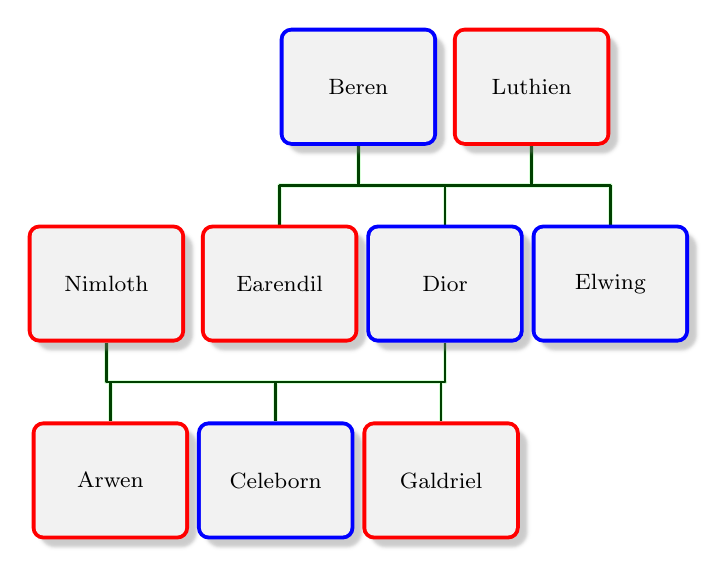
\begin{tikzpicture}
\genealogytree[template=signpost]{
    parent{
      g[female]{Arwen}
      c[male]{Celeborn}
      c[female]{Galdriel}
        p[female]{Nimloth}
    parent{
        c[female]{Earendil}
        g[male]{Dior}
        c[male]{Elwing}
        p[male]{Beren}
        p[female]{Luthien}
}
    }
  }
\end{tikzpicture}

\section{Exotic Features}

\subsection{Epigraph Style}
\subsection*{Chapter 1: Theory of life}
\epigraph{\textit{``Failure will never overtake me if my determination to succeed is strong enough."}}{\textit{Og Mandino}}

\subsection{Minipage}
\fbox{
\begin{minipage}{0.5\linewidth}
\textit{\LaTeX\ typesets a file of text using the TEX program and the \LaTeX\ ``macropackage" for TEX. That is, it processes an input file containing the text of a document with interspersed commands that describe how the text should be formatted. \LaTeX\ files are plain text that can be written in any reasonable editor. In the \LaTeX\ input file, a command name starts with a followed by either (a) a string of letters or (b) a single non-letter. Arguments contained in square brackets, [], are optional while arguments contained in braces, {}, are required. \LaTeX\ is case
sensitive. Enter all commands in lowercase unless explicitly directed to do otherwise.}
\end{minipage}
}

\newpage

\section{Bibliography}
\bibliography{lab.bib}

\end{document}
